% Options for packages loaded elsewhere
\PassOptionsToPackage{unicode}{hyperref}
\PassOptionsToPackage{hyphens}{url}
\PassOptionsToPackage{dvipsnames,svgnames,x11names}{xcolor}
%
\documentclass[
  letterpaper,
  DIV=11,
  numbers=noendperiod]{scrreprt}

\usepackage{amsmath,amssymb}
\usepackage{lmodern}
\usepackage{iftex}
\ifPDFTeX
  \usepackage[T1]{fontenc}
  \usepackage[utf8]{inputenc}
  \usepackage{textcomp} % provide euro and other symbols
\else % if luatex or xetex
  \usepackage{unicode-math}
  \defaultfontfeatures{Scale=MatchLowercase}
  \defaultfontfeatures[\rmfamily]{Ligatures=TeX,Scale=1}
\fi
% Use upquote if available, for straight quotes in verbatim environments
\IfFileExists{upquote.sty}{\usepackage{upquote}}{}
\IfFileExists{microtype.sty}{% use microtype if available
  \usepackage[]{microtype}
  \UseMicrotypeSet[protrusion]{basicmath} % disable protrusion for tt fonts
}{}
\makeatletter
\@ifundefined{KOMAClassName}{% if non-KOMA class
  \IfFileExists{parskip.sty}{%
    \usepackage{parskip}
  }{% else
    \setlength{\parindent}{0pt}
    \setlength{\parskip}{6pt plus 2pt minus 1pt}}
}{% if KOMA class
  \KOMAoptions{parskip=half}}
\makeatother
\usepackage{xcolor}
\setlength{\emergencystretch}{3em} % prevent overfull lines
\setcounter{secnumdepth}{5}
% Make \paragraph and \subparagraph free-standing
\ifx\paragraph\undefined\else
  \let\oldparagraph\paragraph
  \renewcommand{\paragraph}[1]{\oldparagraph{#1}\mbox{}}
\fi
\ifx\subparagraph\undefined\else
  \let\oldsubparagraph\subparagraph
  \renewcommand{\subparagraph}[1]{\oldsubparagraph{#1}\mbox{}}
\fi


\providecommand{\tightlist}{%
  \setlength{\itemsep}{0pt}\setlength{\parskip}{0pt}}\usepackage{longtable,booktabs,array}
\usepackage{calc} % for calculating minipage widths
% Correct order of tables after \paragraph or \subparagraph
\usepackage{etoolbox}
\makeatletter
\patchcmd\longtable{\par}{\if@noskipsec\mbox{}\fi\par}{}{}
\makeatother
% Allow footnotes in longtable head/foot
\IfFileExists{footnotehyper.sty}{\usepackage{footnotehyper}}{\usepackage{footnote}}
\makesavenoteenv{longtable}
\usepackage{graphicx}
\makeatletter
\def\maxwidth{\ifdim\Gin@nat@width>\linewidth\linewidth\else\Gin@nat@width\fi}
\def\maxheight{\ifdim\Gin@nat@height>\textheight\textheight\else\Gin@nat@height\fi}
\makeatother
% Scale images if necessary, so that they will not overflow the page
% margins by default, and it is still possible to overwrite the defaults
% using explicit options in \includegraphics[width, height, ...]{}
\setkeys{Gin}{width=\maxwidth,height=\maxheight,keepaspectratio}
% Set default figure placement to htbp
\makeatletter
\def\fps@figure{htbp}
\makeatother

\usepackage{amsmath}
\usepackage{booktabs}
\usepackage{caption}
\usepackage{longtable}
\KOMAoption{captions}{tableheading}
\makeatletter
\makeatother
\makeatletter
\@ifpackageloaded{bookmark}{}{\usepackage{bookmark}}
\makeatother
\makeatletter
\@ifpackageloaded{caption}{}{\usepackage{caption}}
\AtBeginDocument{%
\ifdefined\contentsname
  \renewcommand*\contentsname{Table of contents}
\else
  \newcommand\contentsname{Table of contents}
\fi
\ifdefined\listfigurename
  \renewcommand*\listfigurename{List of Figures}
\else
  \newcommand\listfigurename{List of Figures}
\fi
\ifdefined\listtablename
  \renewcommand*\listtablename{List of Tables}
\else
  \newcommand\listtablename{List of Tables}
\fi
\ifdefined\figurename
  \renewcommand*\figurename{Figure}
\else
  \newcommand\figurename{Figure}
\fi
\ifdefined\tablename
  \renewcommand*\tablename{Table}
\else
  \newcommand\tablename{Table}
\fi
}
\@ifpackageloaded{float}{}{\usepackage{float}}
\floatstyle{ruled}
\@ifundefined{c@chapter}{\newfloat{codelisting}{h}{lop}}{\newfloat{codelisting}{h}{lop}[chapter]}
\floatname{codelisting}{Listing}
\newcommand*\listoflistings{\listof{codelisting}{List of Listings}}
\makeatother
\makeatletter
\@ifpackageloaded{caption}{}{\usepackage{caption}}
\@ifpackageloaded{subcaption}{}{\usepackage{subcaption}}
\makeatother
\makeatletter
\@ifpackageloaded{tcolorbox}{}{\usepackage[many]{tcolorbox}}
\makeatother
\makeatletter
\@ifundefined{shadecolor}{\definecolor{shadecolor}{rgb}{.97, .97, .97}}
\makeatother
\makeatletter
\makeatother
\ifLuaTeX
  \usepackage{selnolig}  % disable illegal ligatures
\fi
\IfFileExists{bookmark.sty}{\usepackage{bookmark}}{\usepackage{hyperref}}
\IfFileExists{xurl.sty}{\usepackage{xurl}}{} % add URL line breaks if available
\urlstyle{same} % disable monospaced font for URLs
\hypersetup{
  pdftitle={UCSD Equity Gaps},
  pdfauthor={Sarah Nolan},
  colorlinks=true,
  linkcolor={blue},
  filecolor={Maroon},
  citecolor={Blue},
  urlcolor={Blue},
  pdfcreator={LaTeX via pandoc}}

\title{UCSD Equity Gaps}
\author{Sarah Nolan}
\date{2/2/23}

\begin{document}
\maketitle
\ifdefined\Shaded\renewenvironment{Shaded}{\begin{tcolorbox}[borderline west={3pt}{0pt}{shadecolor}, boxrule=0pt, sharp corners, enhanced, interior hidden, frame hidden, breakable]}{\end{tcolorbox}}\fi

\renewcommand*\contentsname{Table of contents}
{
\hypersetup{linkcolor=}
\setcounter{tocdepth}{2}
\tableofcontents
}
\bookmarksetup{startatroot}

\hypertarget{preface}{%
\chapter*{Preface}\label{preface}}
\addcontentsline{toc}{chapter}{Preface}

\markboth{Preface}{Preface}

This is a Quarto book.

To learn more about Quarto books visit
\url{https://quarto.org/docs/books}.

This is currently a placeholder for future content

\bookmarksetup{startatroot}

\hypertarget{data-descriptions}{%
\chapter{Data Descriptions}\label{data-descriptions}}

This book explores data on opportunity gaps at University of California
San Diego (UCSD).

\hypertarget{data-sources}{%
\section{Data Sources}\label{data-sources}}

\hypertarget{sec-UCUES}{%
\subsection{University of California Undergraduate Experience Survey
(UCUES)}\label{sec-UCUES}}

The University of California Undergraduate Experience Survey (UCUES) is
a biennial survey conducted at the UC's nine undergraduate campuses.

For more about UCUES across the UC, and data tables from 2006 onwards,
please see
\href{https://www.universityofcalifornia.edu/about-us/information-center/ucues-data-tables-main}{this
page on UC Infocenter}.

A summary of UCUES at UCSD can be found on UCSD IR website
\href{https://ir.ucsd.edu/undergrad/surveys/index.html}{here}. A
longitudinal comparison of some questions at UCSD can be found
\href{https://tableau.ucsd.edu/\#/views/UCUES_UC_SanDiego/Satisfaction?:iid=1}{here}
for those with an Active Directory login.

\begin{itemize}
\item
  More on group definitions
\item
  More on response rates and sample sizes
\item
  For an interactive view of response rates and sample size see
  \href{https://www.universityofcalifornia.edu/about-us/information-center/student-survey-completion-and-response-rates}{UC
  Infocenter}
\end{itemize}

\hypertarget{sec-UCGSES}{%
\subsection{University of California Graduate Student Experience Survey
(UCGSES)}\label{sec-UCGSES}}

This UC-wide has been conducted once, in 2021. The data table for all UC
campuses is available at the
\href{https://www.universityofcalifornia.edu/about-us/information-center/UCGSES-data-tables}{UC
Infocenter}

UC San Diego had a lower than average response rate for graduate
students in comparison with the other UC campuses.

\begin{figure}

{\centering 

\href{https://www.ucop.edu/institutional-research-academic-planning/_files/survey-documents-graduate/ucgses-2021-administration-report.pdf}{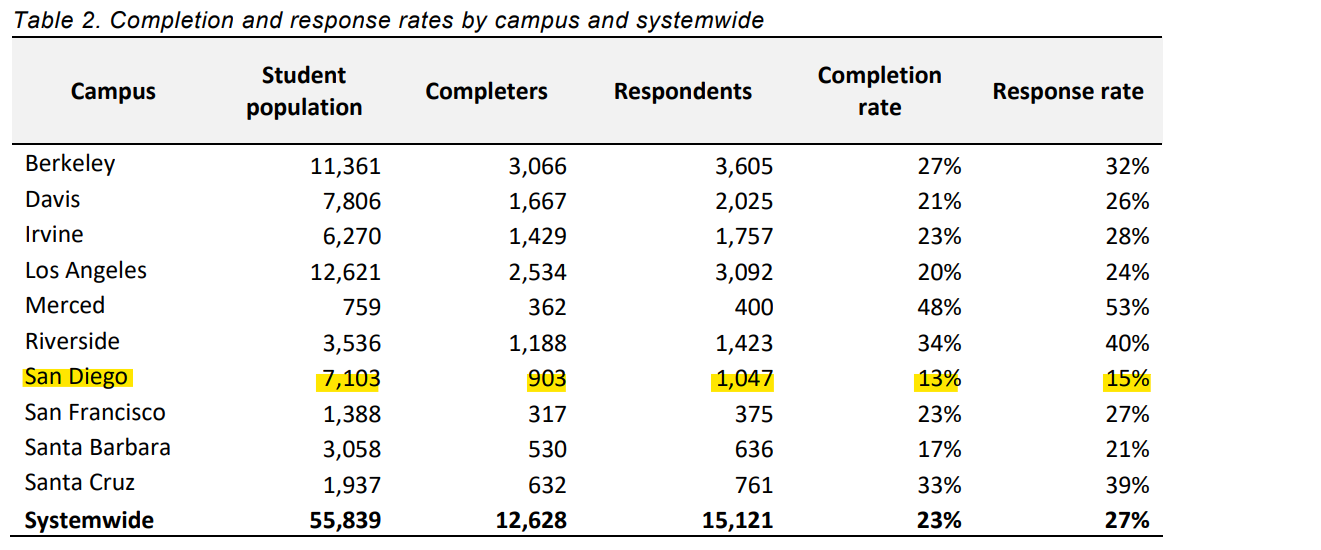
\includegraphics{./viz/UCGSES_rr_table.png}}

}

\caption{UCGSES 2021}

\end{figure}

\hypertarget{graduate-student-category-definitions-response-rates}{%
\subsubsection{Graduate Student Category Definitions, Response
Rates}\label{graduate-student-category-definitions-response-rates}}

This section currently features screenshots from the UCOP Info Center
\href{https://www.universityofcalifornia.edu/about-us/information-center/UCGSES-survey}{UCGSES
2021 Survey Dashboard} under the ``Student Profile'' tab and filtered to
Campus: UC San Diego and the respective student characteristics.

\hypertarget{first-generation}{%
\paragraph{First Generation}\label{first-generation}}

Future versions of this document will include population figures f
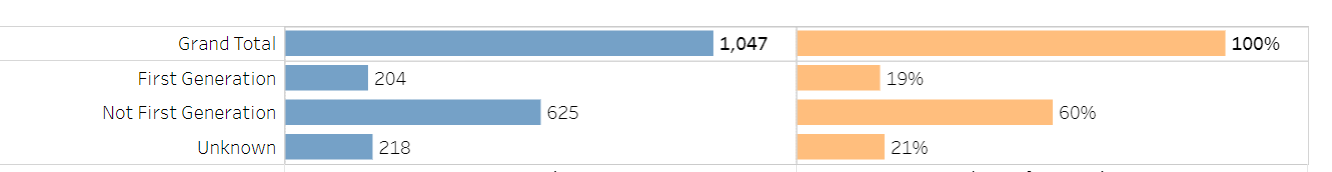
\includegraphics{./viz/intro/ucgses_first_gen.png}

\hypertarget{additional-surveys}{%
\subsection{Additional Surveys}\label{additional-surveys}}

Future versions of this report may include information from other
student surveys

\textbf{Undergraduates}

\begin{itemize}
\item
  The CIRP Freshman Survey /New Transfer Survey
\item
  Your College First Year Survey
\item
  College Senior Survey
\item
  Post Baccalaureate
\item
  Cost of Attendance Survey
\end{itemize}

\textbf{Graduate Students} UCSD data is available
\href{https://grad.ucsd.edu/about/grad-data/surveys/index.html}{here}

\begin{itemize}
\item
  Graduate Student Experience in the Resarch University (gradSERU)
\item
  Graduate Student Well-Being Survey
\item
  Graduate and Professional Student Experience and Satisfaction (GPSES)
\item
  Graduate Student Exit Survey
\item
  Cost of Attendance Survey
\end{itemize}

\bookmarksetup{startatroot}

\hypertarget{academic-outcomes}{%
\chapter{Academic Outcomes}\label{academic-outcomes}}

This chapter explores equity gaps in graduation rates, retention, and
GPA at graduation.

These visuals draw from a wealth of data - readers interested in a
deeper exploration can turn to UCSD's Institutional Research Website.
For more on these trends in the UC system as a whole, please see the
University of California Office of the President's Accountability
Report, Chapter 3 for Undergraduate Success

\begin{itemize}
\item
  \href{https://ir.ucsd.edu/undergrad/stats-data/ug-retention.html}{UCSD
  IR Undergraduate Graduation and Retention Rates}
\item
  \href{https://ir.ucsd.edu/undergrad/stats-data/ug-degree.html}{UCSD IR
  Undergraduate GPA}
\item
  \href{https://accountability.universityofcalifornia.edu/2022/chapters/chapter-3.html}{All
  UC Accountability , Undergraduate Success, 2022}
\end{itemize}

\hypertarget{graduation-rates}{%
\subsection{Graduation Rates}\label{graduation-rates}}

\hypertarget{first-time-first-years}{%
\subsubsection{First-Time-First-Years}\label{first-time-first-years}}

First, we examine the percentage of First-Time-First-Year (FTFY)
students who graduate within six years or less of starting at UCSD. The
below visual shows six year graduation rates for the entering cohort of
2016. Overall, 85\% of FTFY students entering in 2016 graduated in six
years or less. The proportion of students who recieve Pell Grants, and
First Generation students, have slightly lower graduation rates of 83\%
and 84\% respectively.

The largest equity gaps emerge when considering Race and Ethnicity.
Hispanic / Latinx, African American, and American Indian students each
have lower than average graduation rates, of 81\%, 78\%, and 74\%
respectively.

\includegraphics{./C1_Academic_Outcomes_files/figure-pdf/ftfy_six_2016-1.pdf}

Examining the proportion of students who graduate within four years or
less shows a similar pattern of equity gaps, however the divergence
between student groups grows larger. For the most recent entry cohort
available, 2018, about 73\% of students graduate in four years or less.
However, that proportion drops to 55\%, just over half, for African
American students in that entering cohort, and 12\% for Hispanic/Latinx.

\textbf{Need to document change over time- there's a small number of
American Indian students and proportions are more variable year over
year}

\includegraphics{./C1_Academic_Outcomes_files/figure-pdf/ftfy_four_2018-1.pdf}

\hypertarget{transfer-students}{%
\subsubsection{Transfer Students}\label{transfer-students}}

Overall, the size of equity gaps between transfer students is smaller,
Transfer student graduation rates within four years or fewer is about
87\% for all Transfer students.

\includegraphics{./C1_Academic_Outcomes_files/figure-pdf/t_four_2018-1.pdf}

When considering equity gaps in ``on-time'' graduation -two years or
less- the overall average falls to about 57\%. However, the difference
between student groups relative to this average is relatively small,
with the exception of African American transfer students, 46\% of whom
entering in 2020 graduated within two years or less.

\includegraphics{./C1_Academic_Outcomes_files/figure-pdf/t_two_2020-1.pdf}

\hypertarget{one-year-retention}{%
\subsection{One Year Retention}\label{one-year-retention}}

Retention rates over the first year are on average very high, with 93\%
of FTFY students remaining enrolled after the first year, and 92-93\% of
Transfer students. African American students have lower retention rates,
at 83\% for FTFY students.

** Change over Time is Important and needs to be considered- especially
for American Indian students **

\includegraphics{./C1_Academic_Outcomes_files/figure-pdf/ftfy_ret_2021-1.pdf}

\includegraphics{./C1_Academic_Outcomes_files/figure-pdf/t_ret_2021-1.pdf}

\hypertarget{gpa}{%
\subsection{GPA}\label{gpa}}

The below visual provides just one view of GPA, the GPA of students at
graduation, specifically the percent of students graduating with less
than a 3.0 GPA (2.0-2.99)

Department/ Major is one unmeasured component in these comparisons,
where internal analyses like Academic Program Review offer more
sophisticated analyses. However, the following visual shows what is
possible with publicly available data.

This visual also does not include students who drop or stop out prior to
graduating.

About 15\% of all graduating undergraduates in 2022 had a GPA below 3.0
at graduation. However, a higher proportion of Transfer students,
African American, and Hispanic/Latinx students graduate with a GPA below
3.0, 19\%, 26\%, and 25\% respectively.

\includegraphics{./C1_Academic_Outcomes_files/figure-pdf/gpa_2022-1.pdf}

\hypertarget{graduate-students}{%
\section{Graduate Students}\label{graduate-students}}

A wealth of department level data can be found at the
\href{https://grad.ucsd.edu/about/grad-data/completion-rates.html}{UCSD
Graduate Data website}. The below visual offers a high level comparison
of completion rates for doctoral students, making a comparison between
members of Underrepresented Groups (African American, Hispanic/Latinx,
and/or American Indian, domestic), members of represented groups,
domestic, and International students. Completion rates within 10 years
for entry cohorts between 2009-2011 range from just 64\% of URG students
to 81\% of international students.

\hypertarget{year-completion-rates}{%
\subsection{10 Year Completion Rates}\label{year-completion-rates}}

\includegraphics{./C1_Academic_Outcomes_files/figure-pdf/grad_10-1.pdf}

\bookmarksetup{startatroot}

\hypertarget{affordable-learning-and-financial-support}{%
\chapter{Affordable Learning and Financial
Support}\label{affordable-learning-and-financial-support}}

This is a chapter about affordable learning and financial support at
University of California San Diego. The first two sections focus on
undergraduate and graduate student survey responses. The third section
explores results from a one-time survey of undergraduate students on
their experiences with buying course materials. Finally, an appendix
provide the number of respondents for each survey question by student
group.

This section covers a few questions prioritized by the Affordable
Learning and Financial Support collective impact working group.

Please refer to Section~\ref{sec-UCUES} for more information on UCUES.
For readers affiliated with UCSD and a working Active Directory login, a
few longitudinal questions can be explored on
\href{https://tableau.ucsd.edu/\#/views/UCUES_UC_SanDiego/Affordability?:iid=1}{Instiutional
Research's Dashboard}

\hypertarget{food-security}{%
\subsection{Food Security}\label{food-security}}

Student respondents are assigned a food security level: very low food
security, low food security, or food secure, based on their responses to
six questions.

For more information on this measure, please visit
\href{https://www.universityofcalifornia.edu/sites/default/files/measuring-food-insecurity.pdf}{UCOP
Measuring Food Insecurity}

\hypertarget{food-security-over-time}{%
\subsubsection{Food Security over Time}\label{food-security-over-time}}

These visuals display the combined percentage of respondents who are
``food insecure'' or ``very food insecure''. For example, in 2022, 42\%
of UCSD undergraduate respondents were classified as food insecure or
very food insecure. This means the remaining 58\% of respondents were
food secure.

The percent of undergraduates who are food insecure has remained
relatively stable over time. UCSD's food insecurity rates are slightly
lower or equal to the overall UC system rate for this time period.

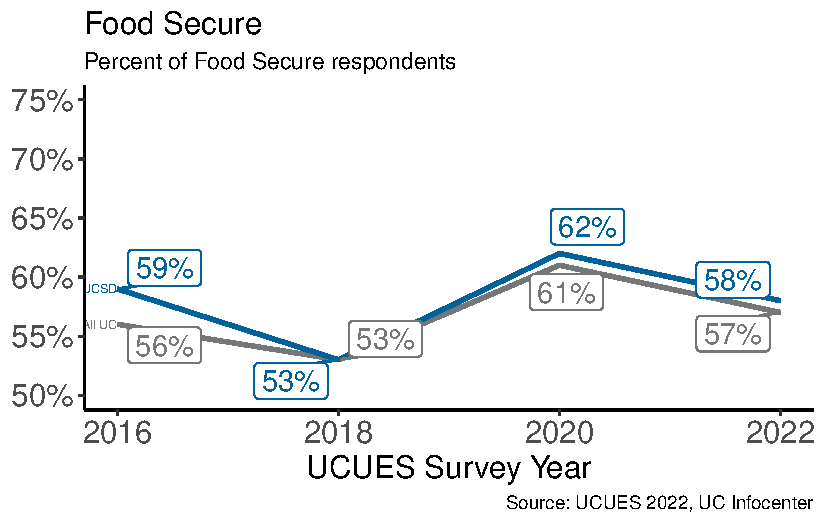
\includegraphics{./C2_Affordable_Learning_files/figure-pdf/food_secure_ug_overtime-1.pdf}

\hypertarget{food-security-differences-by-group}{%
\subsubsection{Food Security Differences by
Group}\label{food-security-differences-by-group}}

Focusing on UCSD students in 2022, we find that there are significant
differences by student group. In comparison to the all-undergraduate
proportion of 42\% food insecure, the proportion is higher for Pell
Grant Recipients (51\%), First Generation students (52\%), African
American students (55\%), Hispanic/Latinx students (52\%) and American
Indian students (50\%).

Overall, there is \textasciitilde18 percentage point difference between
the group with the lowest food insecurity - domestic, White students
(37\%) and that with the highest, domestic, African American students
(55\%).

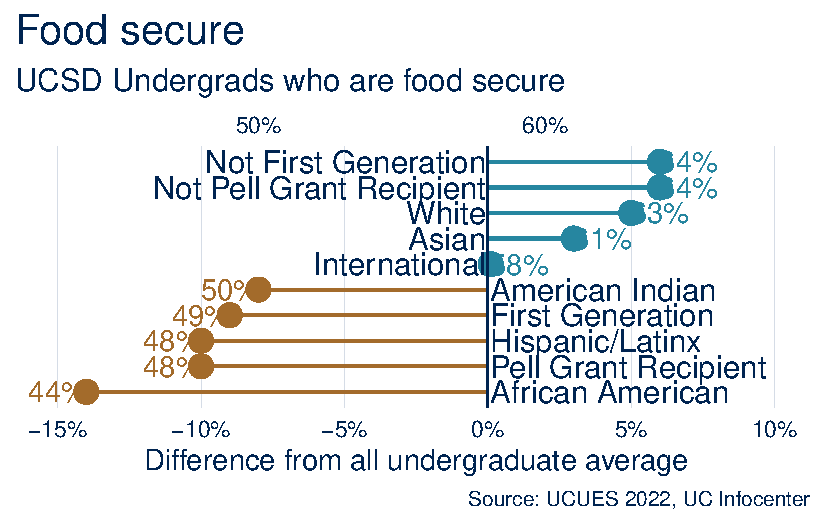
\includegraphics{./C2_Affordable_Learning_files/figure-pdf/food_secure_ug_differences_2022-1.pdf}

\hypertarget{housing-costs}{%
\subsection{Housing Costs}\label{housing-costs}}

The prioritization poll selected two housing questions from the most
recent UCUES 2022 wave- these questions had not been asked previously.
There are other housing related questions that future versions of this
document can add to provide historical context.

The question block prompts: ``For the following statements, please
indicate whether the statement was never true, sometimes true, or often
true for you during the current academic year:''

``I was unable to pay all the cost of my housing on time.''

``I was worried I would not have enough money to cover the cost of my
housing''

Respondents could select ``Never True'', ``Sometimes True'' or ``Often
True.'' For consistency in selecting negative responses - we focus on
``Sometimes True'' and ``Often True'' responses- meaning that
respondents were unable to pay and worried about their housing costs.

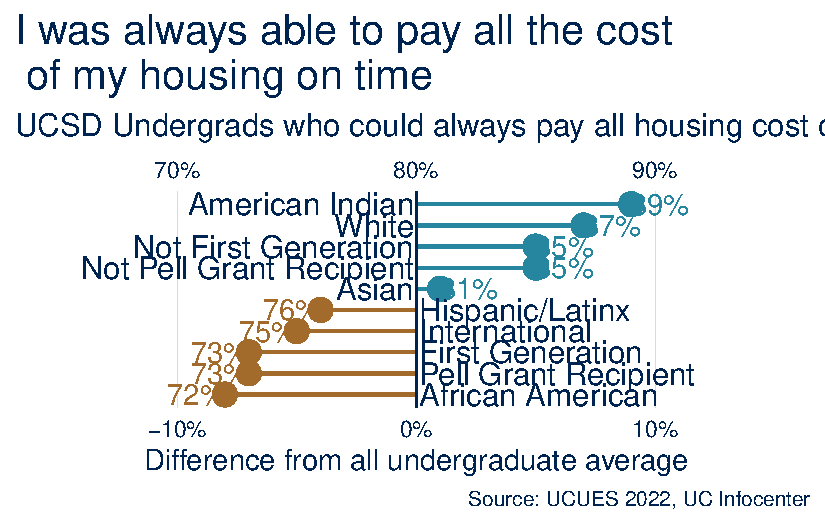
\includegraphics{./C2_Affordable_Learning_files/figure-pdf/unable_pay_house_ug_diff_2022-1.pdf}

About 20\% of students were sometimes or often unable to pay on time.
This proportion is slightly lower than the UC average of 23\% of
students unable to pay (not pictured).

Within UCSD, the proportion of students unable to pay on time ranges
from 28\% for African American students to 11\% for American Indian
students, a 17 percentage point difference.

The proportion of students who worry about paying housing costs is
higher. Overall 46\% worry -similar to the UC average of 45\%. However,
there is a wide range by student groups at UCSD, from 68\% of Pell Grant
students worrying, to only 44\% of those who don't receive Pell, a
difference of over 20 percentage points. The proportions for
Hispanic/Latinx and African American students who worry is also high,
around 62\%.

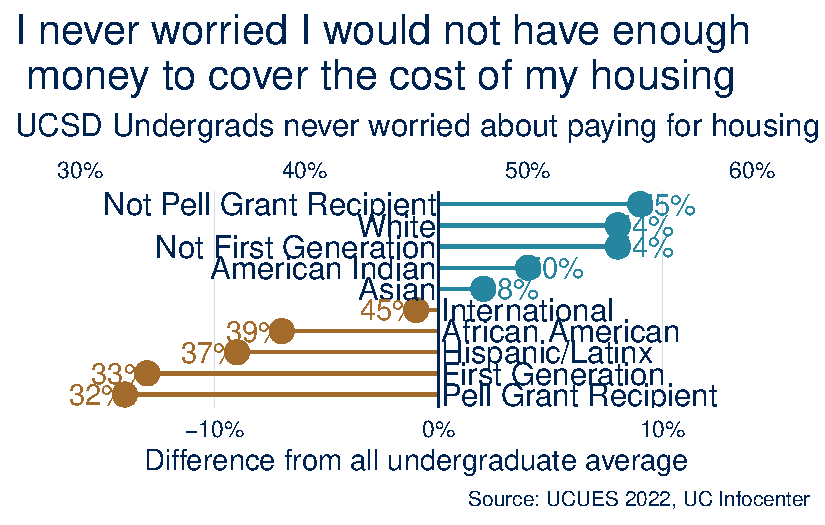
\includegraphics{./C2_Affordable_Learning_files/figure-pdf/worried_pay_house_ug_diff_2022-1.pdf}

\hypertarget{worried-about-debtfinances}{%
\subsection{Worried about
Debt/Finances}\label{worried-about-debtfinances}}

UCUES has asked ``How often during the past academic year have you:
Worried about debt and financial circumstances?'' since 2014.

The question has six possible responses -three coded negative: Very
Often, Often, Somewhat Often, and three as more positive: Occasionally,
Rarely, Never. We focus here on the negative responses.

Overall, UCSD's students are similar to or slightly less worried than
the UC average, with the percent of students worried falling for both in
2022.

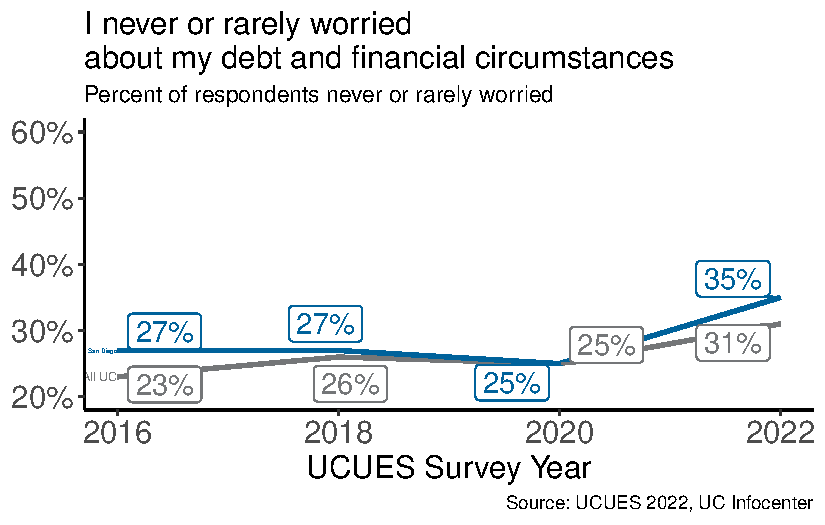
\includegraphics{./C2_Affordable_Learning_files/figure-pdf/worried_debt_ug_overtime-1.pdf}

It's notable that while 2022 saw a decrease in students worried, stark
differences remain by student group,

\includegraphics{./C2_Affordable_Learning_files/figure-pdf/worried_debt_ug_diff_2022-1.pdf}

\hypertarget{manageable-costs}{%
\subsection{Manageable Costs}\label{manageable-costs}}

Forty-two percent of students somewhat disagree, disagree, or strongly
disagree that the total cost of attending UCSD is manageable, given the
the grants and scholarships they receive. Over the past four waves of
UCUES, UCSD has had slightly higher proportions of students disagree
that it is manageable than the UC average.

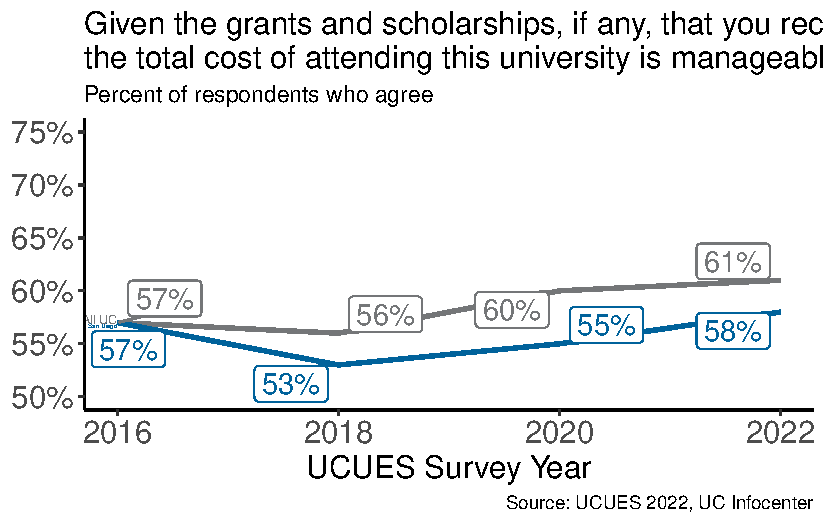
\includegraphics{./C2_Affordable_Learning_files/figure-pdf/manageable_ug_overtime-1.pdf}

Interestingly, the consistent gaps by student group observed for other
affordability questions partially reverse in this question.

Those who do not receive Pell Grants, and not First Generation students
have a higher proportion of negative responses. 49\% of students not
receiving Pell Grants disagree that the cost of UCSD is manageable,
compared to 30\% of Pell Grant recipients.

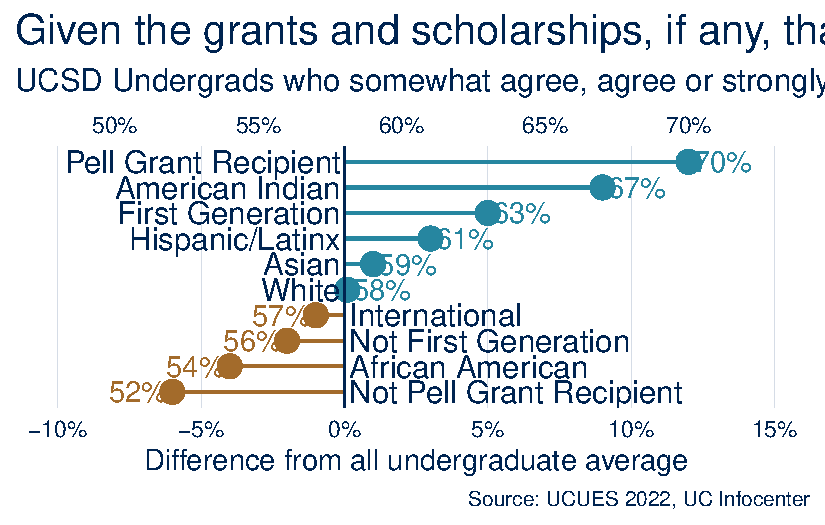
\includegraphics{./C2_Affordable_Learning_files/figure-pdf/manageable_ug_2022-1.pdf}

\hypertarget{additional-ucues-questions-related-to-affordability.}{%
\subsection{Additional UCUES Questions related to
Affordability.}\label{additional-ucues-questions-related-to-affordability.}}

These questions are also available on the 2022 UCUES for further
exploration.

\begin{itemize}
\tightlist
\item
  Overall, I feel the education is affordable at my campus
\item
  How satisfied are you with the following aspect of your campus
  experiences/education? Value of your education for the price you are
  paying.
\item
  How concerned have you been about paying for your undergraduate
  education up to now?
\item
  \ldots Next Year?
\item
  How often during the past academic year have you: cut down on personal
  / recreational spending to help pay for college expenses?
\end{itemize}

\hypertarget{graduate-students-1}{%
\section{Graduate Students}\label{graduate-students-1}}

There have been fewer consistent questions asked to graduate students
over time, and slightly different student groups are available in
publicly available data. See data descriptions for more detail. The
following draw from the UC Graduate Student Experience Survey in 2021,
with the exception of Food Security, which includes data from the 2016
Graduate Student Wellbeing Survey. Please refer to
Section~\ref{sec-UCGSES} for more on UCGSES.

\hypertarget{food-security-1}{%
\subsection{Food Security}\label{food-security-1}}

For the two waves available for Graduate Students, UCSD has similar
rates of food insecurity in comparison with the UC average.

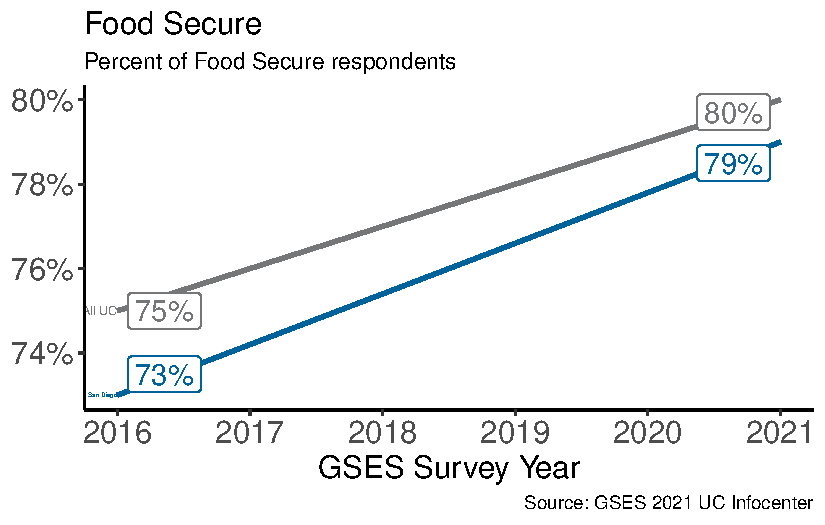
\includegraphics{./C2_Affordable_Learning_files/figure-pdf/food_g_overtime-1.pdf}

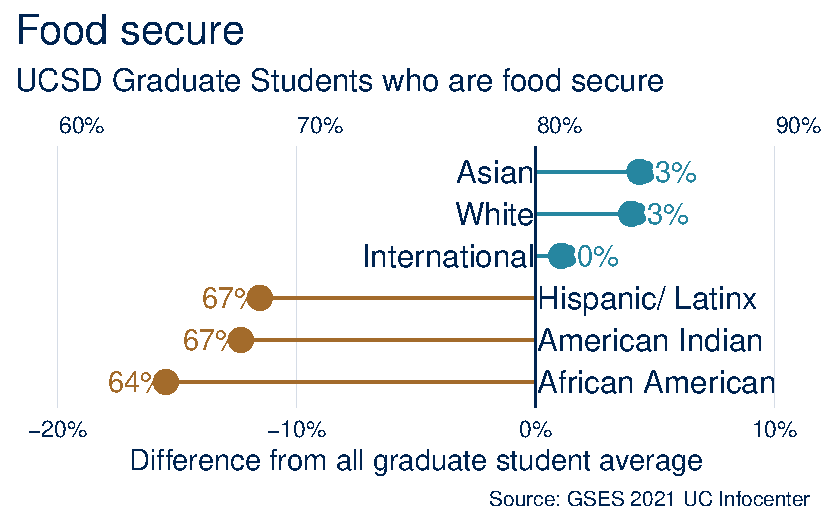
\includegraphics{./C2_Affordable_Learning_files/figure-pdf/food_g_2021-1.pdf}

\hypertarget{financial-hardship-has-impeded-my-success-in-my-program.}{%
\subsection{Financial hardship has impeded my success in my
program.}\label{financial-hardship-has-impeded-my-success-in-my-program.}}

Graduate students were asked to indicate their agreement with this
statement ``Financial Hardship has impeded my success in my program.''
Students who selected ``Strongly Agree'' ``Agree'' and ``Somewhat
Agree'' were coded as ``negative'' responses.

While about 36\% of students agreed that financial hardship had impeded
their success, similar to the all-UC rate of 35\% (not pictured), that
number rises to 52\% for Hispanic/Latinx students - and First
Generation, LGBT, African American, Doctoral students, and International
students also have higher levels of agreement than average.

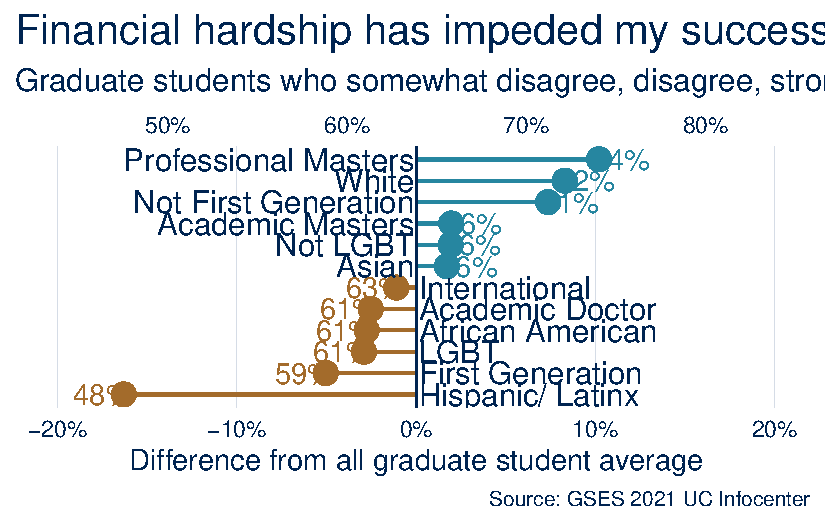
\includegraphics{./C2_Affordable_Learning_files/figure-pdf/hardship_g_2021-1.pdf}

\hypertarget{ive-been-concerned-about-money-lately.}{%
\subsection{I've been concerned about money
lately.}\label{ive-been-concerned-about-money-lately.}}

This question continues the format of the previous, with similar
patterns of differences between groups. The UCSD proportion of students
who agree they are concerned about money lately is about 66\%, similar
the all-UC proportion of 67\%.

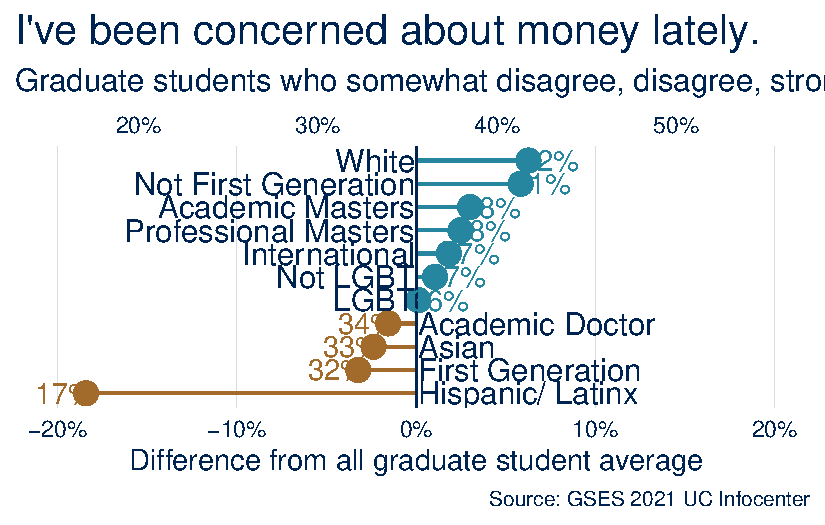
\includegraphics{./C2_Affordable_Learning_files/figure-pdf/concerned_g_2021-1.pdf}

\hypertarget{im-confident-in-my-financial-situation.}{%
\subsection{I'm confident in my financial
situation.}\label{im-confident-in-my-financial-situation.}}

For this question, ``Strongly Disagree,'' ``Disagree'', and ``Somewhat
Disagree'' were considered negative responses. There is a divergence
between UCSDand the all UC rate, with a lower proportion of UCSD
students disagreeing - 31\% vs 34\% of all UC respondents.

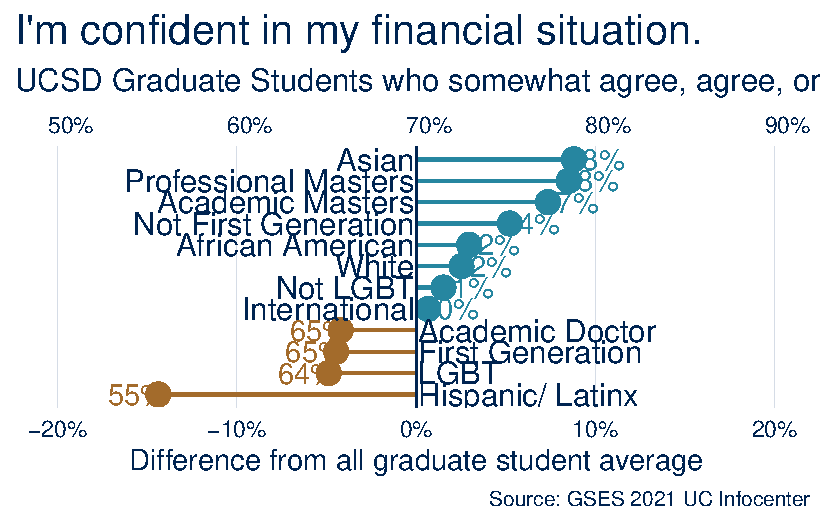
\includegraphics{./C2_Affordable_Learning_files/figure-pdf/confident_g_2021-1.pdf}

\hypertarget{i-can-get-by-financially-without-having-to-cut-back-on-too-many-of-the-things-that-are-important-to-me.}{%
\subsection{I can get by financially without having to cut back on too
many of the things that are important to
me.}\label{i-can-get-by-financially-without-having-to-cut-back-on-too-many-of-the-things-that-are-important-to-me.}}

For this question, ``Strongly Disagree,'' ``Disagree'', and ``Somewhat
Disagree'' were considered negative responses. Again, the proportion for
all UCSD students (32\%) is relatively similiar to the all UC proportion
(34\%)

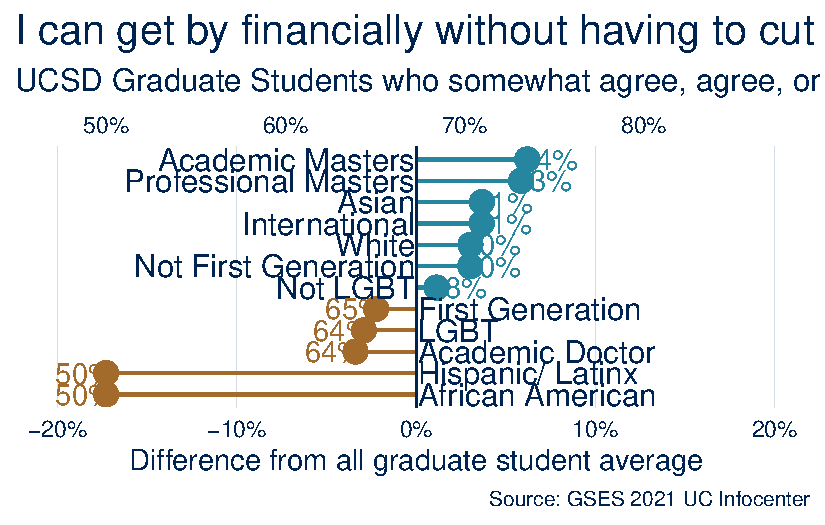
\includegraphics{./C2_Affordable_Learning_files/figure-pdf/getby_g_2021-1.pdf}

\hypertarget{affordable-and-open-course-materials}{%
\section{Affordable and Open Course
Materials}\label{affordable-and-open-course-materials}}

The following paragraphs are quoted verbatim from the Affordable / Open
course Materials Report - May 2022.

In November 2021, a team from the Library and the Teaching + Learning
Commons (April Cha, Dani Cook, Leah Klement, Lisa Martin, and Allegra
Swift) fielded a population-level survey about student experiences with
obtaining and using course materials.

With help from William Armstrong in Institutional Research, we sent
32,827 survey invitations to UC San Diego undergraduate students. 2,153
students consented and participated in the survey, for a response rate
of 6.6\%. Demographic characteristics of both the full population and
responding population fell within 2 percentage points of each other for
college, major department, race, first-generation status, and Pell
eligibility. Female students were overrepresented in the responding
population, and transfer students were slightly underrepresented in
respondents.

Questions on the survey related to student spending on course materials
in fall 2021; how students pay for course materials; student strategies
when they don't own course materials; student interest in an inclusive
access program; academic, social, and basic needs impacts of course
materials cost and access; and format preference.

\hypertarget{student-spending}{%
\subsection{Student Spending}\label{student-spending}}

The largest number of students reported spending under \$100 (38\%) on
course materials in fall 2021. However, a similar number of students
reported spending between \$100 and \$199 dollars (33.4\%), and the
remaining 29\% reported spending over \$200 on course materials. A small
number of students (.7\%) reported spending more than \$600. One
representative statement was, ``I think it's expected to spend money on
courses and textbooks, it just hits lower-income students harder for
obvious reasons.''

Some free-text responses mention departments that already keep material
costs low, including CSE and political science. These may be areas to
reach out to for more information.

We also investigated if there was a relationship between how much
students spent on course materials and their usage. There does appear to
be a correlation between cost and usage (p\textless.001). In general,
students reported using most (above 80\%) of their required course
materials across categories (31.2\% of respondents). However, there were
numerous students who reported that they used below 50\% of their
assigned course materials in a quarter, and the qualitative data
represented that some students felt frustrated that they were assigned
materials that they did not use in the course. Student comments related
to this topics included: ``I do not mind buying course materials if it
is used for at least 50\% of the course. Otherwise it feels like a
waste'' and ``It would be great if professors specified beforehand if we
will actually be using the textbook. Sometimes it's listed as required
but never used.'' This was the second-most commented-on topic in the
qualitative data.

Of students who spent below \$100, 10\% of them reported never using any
of their course materials. However, the preponderance of students in
this category (31.4\%) reported using 80\% or more of their assigned
course materials.

For the top spenders (students who spend \$600 or more), most (56.25\%)
reported using most of their materials, and all reported using at least
some.

Latinx students were slightly more likely to spend in the higher price
bands than other groups.

By a significant margin, most students reported that they paid for their
course materials through money provided by family, friends, or
caregivers (43.3\%), followed by money they had earned themselves
(29.9\%) and grants (12.7\%). The chart below demonstrates differences
across racial categories:

\begin{figure}

{\centering 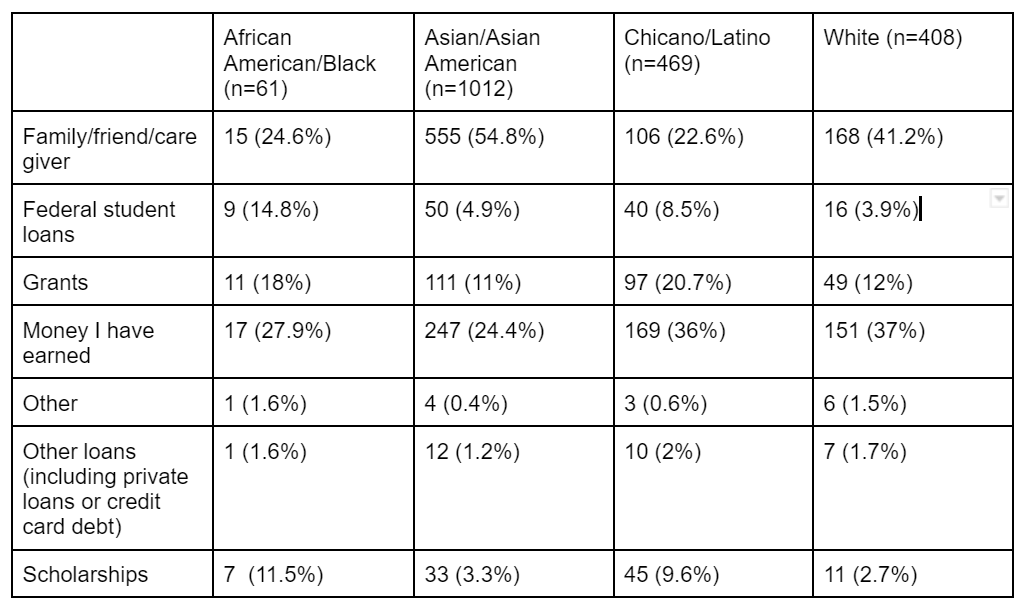
\includegraphics{./viz/alfs/AOCM_student_spending.png}

}

\caption{Student Source of Payment for Course Materials: Race/Ethnicity}

\end{figure}

White and Asian/Asian American students are much more likely to report
having family, friend, or caregiver support for purchasing course
materials.

Similar disparate impacts were demonstrated due to first-generation
status:

\begin{figure}

{\centering 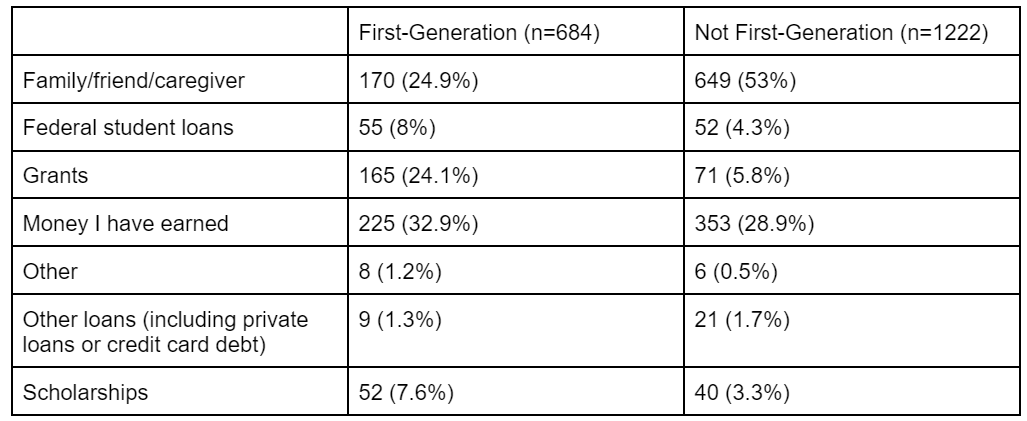
\includegraphics{./viz/alfs/AOCM_student_spending_1g.png}

}

\caption{Student Source of Payment for Course Materials: First
Generation Status}

\end{figure}

80\% of students reported having to purchase access codes (one-time-use
codes to access homework sets, quizzes, or other ancillary materials)
during their time at UC San Diego. There does not appear to be a
relationship between student major and access code purchasing,
indicating that this is a broadly utilized type of course material
across disciplines. It is also unclear from our data if access codes are
more often used in major courses or in general education.

By far, access codes was the area that students shared the most about in
the qualitative data. ``Frustration'' was the most commonly used
adjective. One student shared, ``Purchasing access codes to complete
homework for a grade is ridiculous. We already pay tuition, we shouldn't
have to pay hundreds for our grades too.''

\hypertarget{strategies-for-obtaining-course-materials}{%
\subsection{Strategies for Obtaining Course
Materials}\label{strategies-for-obtaining-course-materials}}

96\% of students who answered the survey indicated that they had
attempted to reduce course material costs during their UC San Diego
career. 64\% of students shared that they had downloaded a ``free''
textbook from the Internet (we did not ask about the legal status of the
copy) and almost half of students (49\%) relying on materials that
course instructors provided through Canvas or other means.

The most common reason given for seeking alternative methods to buying a
course material was because of the cost of the book, followed by because
only a small portion of the material was used in class. Only a small
number of students (1.8\%) indicated familiarity with library course
reserves.

\hypertarget{inclusive-access-program-interest}{%
\subsection{Inclusive Access Program
Interest}\label{inclusive-access-program-interest}}

66\% of students said they would be interested in a standardized fee for
materials from the Bookstore (though many indicated they wanted to know
more about the cost). Without having additional details, 95\% of
respondents believed that a reasonable cost for such a program would be
under \$150 per quarter.

\hypertarget{basic-needs-impacts}{%
\subsection{Basic Needs Impacts}\label{basic-needs-impacts}}

27\% of students who responded to the survey indicated that they had to
make a choice between purchasing course materials and basic needs.

41.6\% of Pell-eligible students who answered the question about basic
needs reported having to make a decision between course materials and
basic needs.

In comparison, 20.3\% of non-Pell-eligible students who answered this
question reported having to make a decision between course materials and
basic needs.

The most commonly reported basic need impacted was access to food,
followed by mental health/well-being and utilities.

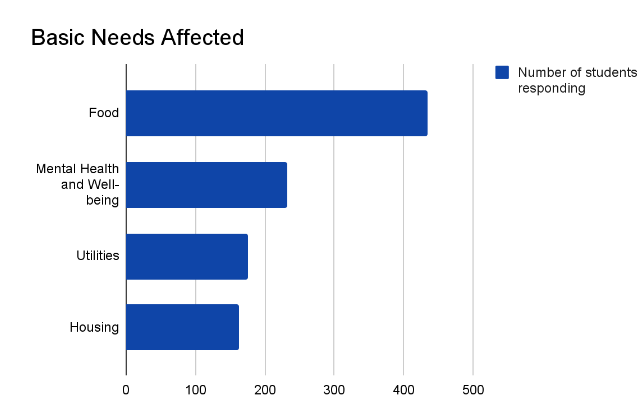
\includegraphics{./viz/alfs/AOCM_basic_needs.png}

\hypertarget{academic-and-social-impacts}{%
\subsection{Academic and Social
Impacts}\label{academic-and-social-impacts}}

The survey also asked questions about how access to course materials
impacted their academic and social lives at UC San Diego.

14.2\% of students overall reported that lack of access to course
materials strongly impacted their understanding of key course concepts.
This impact was felt variably across demographic categories. Notably,
20.9\% of Latinx students reported a strong impact on their
understanding of course concepts, while only 9.6\% of white students
reported a strong impact.

Overall, 10.9\% of students reported that a lack of access to course
materials has affected their feeling of belonging in their course or
major. Again, this impact was felt variably across demographic
categories. 28.1\% of black students reported a strong impact, while
only 7.7\% of white students reported the same. This was also true
across low-income students (as identified by Pell-grant eligibility),
where 41.6\% of Pell-eligible students reported an impact on feelings of
belonging, in contrast to 29\% of non-Pell-eligible students.

\hypertarget{format-preferences}{%
\subsection{Format Preferences}\label{format-preferences}}

Students were queried for their format preferences for course materials.
There is a strong belief that students prefer electronic sources;
however, our survey results indicate that may not be an accurate belief.
While students preferred PDFs or other digital documents, this was
closely followed by professional printed textbooks. The below chart
demonstrates the rank-ordered student preferences.

\begin{figure}

{\centering 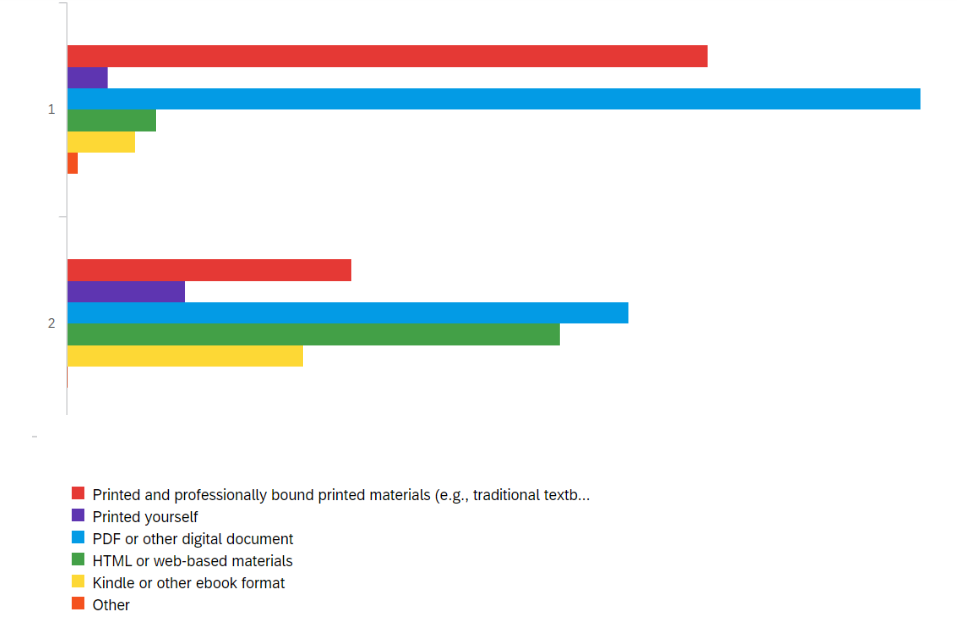
\includegraphics{./viz/alfs/AOCM_format_pref.png}

}

\caption{Student Format Preferences}

\end{figure}

\hypertarget{appendix-response-rates-by-question}{%
\section{Appendix: Response Rates by
Question}\label{appendix-response-rates-by-question}}

\hypertarget{undergraduates-ucues}{%
\subsection{Undergraduates: UCUES}\label{undergraduates-ucues}}

\includegraphics{./C2_Affordable_Learning_files/figure-pdf/ucues_rr_gt-1.png}

\hypertarget{graduate-students-ucgses}{%
\subsection{Graduate Students (UCGSES)}\label{graduate-students-ucgses}}

\includegraphics{./C2_Affordable_Learning_files/figure-pdf/ucgses_rr_gt-1.png}

\bookmarksetup{startatroot}

\hypertarget{academic-experiences}{%
\chapter{Academic Experiences}\label{academic-experiences}}

This is a chapter about academic outcomes at UCSD

\hypertarget{overall-academic-experience}{%
\subsection{Overall Academic
Experience}\label{overall-academic-experience}}

\includegraphics{./C3_Academic_Experiences_files/figure-pdf/overall_ac-1.pdf}

\hypertarget{faculty-knew-your-name}{%
\subsection{Faculty knew your name}\label{faculty-knew-your-name}}

\includegraphics{./C3_Academic_Experiences_files/figure-pdf/fac_name-1.pdf}

\hypertarget{faculty-are-genuinely-committed-to-promoting-respect-for-and-understanding-of-group-differences-at-uc}{%
\subsection{Faculty are genuinely committed to promoting respect for and
understanding of group differences at
UC}\label{faculty-are-genuinely-committed-to-promoting-respect-for-and-understanding-of-group-differences-at-uc}}

\includegraphics{./C3_Academic_Experiences_files/figure-pdf/fac_respect-1.pdf}

\hypertarget{graduate-students-2}{%
\section{Graduate Students}\label{graduate-students-2}}

\hypertarget{quality-of-teaching-in-program}{%
\subsection{Quality of Teaching in
Program}\label{quality-of-teaching-in-program}}

\includegraphics{./C3_Academic_Experiences_files/figure-pdf/qual_teach-1.pdf}

\hypertarget{specialization-teaching}{%
\subsection{Specialization Teaching}\label{specialization-teaching}}

\includegraphics{./C3_Academic_Experiences_files/figure-pdf/qual_teach_spec-1.pdf}

\hypertarget{i-feel-echod-by-the-faculty}{%
\subsection{I feel echod by the
faculty}\label{i-feel-echod-by-the-faculty}}

\includegraphics{./C3_Academic_Experiences_files/figure-pdf/inlcuded_fac-1.pdf}

\hypertarget{my-culture-is-respected-by-the-faculty}{%
\subsection{My culture is respected by the
faculty}\label{my-culture-is-respected-by-the-faculty}}

\includegraphics{./C3_Academic_Experiences_files/figure-pdf/fac_cul-1.pdf}

\hypertarget{response-rates}{%
\section{Response Rates}\label{response-rates}}

\hypertarget{ucues}{%
\subsubsection{UCUES}\label{ucues}}

\captionsetup[table]{labelformat=empty,skip=1pt}
\begin{longtable}{r|rrr}
\caption*{
{\large UCSD Student Response Counts} \\ 
{\small UCUES 2022}
} \\ 
\toprule
\multicolumn{1}{l}{} & \multicolumn{2}{c}{UCUES Questions} &  \\ 
\cmidrule(lr){2-3}
\multicolumn{1}{l}{} & Faculty are ...group differences at UCSD & Had a class in which the professor knew or learned your name & Overall academic experience \\ 
\midrule
\multicolumn{1}{l}{All} \\ 
\midrule
All & 4176 & 9465 & 9548 \\ 
\midrule
\multicolumn{1}{l}{First Gen} \\ 
\midrule
First Generation & 1549 & 3494 & 3532 \\ 
Not First Generation & 2519 & 5718 & 5761 \\ 
\midrule
\multicolumn{1}{l}{Pell} \\ 
\midrule
Not Pell Grant Recipient & 2589 & 5875 & 5919 \\ 
Pell Grant Recipient & 1587 & 3590 & 3629 \\ 
\midrule
\multicolumn{1}{l}{Race} \\ 
\midrule
African American & 121 & 284 & 286 \\ 
American Indian & 23 & 38 & 38 \\ 
Asian & 1690 & 3884 & 3919 \\ 
Hispanic/Latinx & 905 & 2085 & 2100 \\ 
International & 481 & 1076 & 1095 \\ 
White & 848 & 1854 & 1864 \\ 
\midrule
\multicolumn{1}{l}{Applicant Level} \\ 
\midrule
First-Time First Year & NA & 7381 & NA \\ 
Transfer & NA & 2084 & NA \\ 
\bottomrule
\end{longtable}

\includegraphics{./C3_Academic_Experiences_files/figure-pdf/ucues_rr_gt-1.png}

\hypertarget{gses}{%
\subsection{GSES}\label{gses}}

\captionsetup[table]{labelformat=empty,skip=1pt}
\begin{longtable}{r|rrr}
\caption*{
{\large UCSD Student Response Counts} \\ 
{\small UCGSES 2021}
} \\ 
\toprule
\multicolumn{1}{l}{} & \multicolumn{3}{c}{UCGSES Questions} \\ 
\cmidrule(lr){2-4}
\multicolumn{1}{l}{} & I feel included by... the faculty & Quality of teaching in your area of specialization & Quality of teaching in your program \\ 
\midrule
\multicolumn{1}{l}{All} \\ 
\midrule
All & 913 & 975 & 996 \\ 
\midrule
\multicolumn{1}{l}{First Gen} \\ 
\midrule
First Generation & 376 & 368 & 374 \\ 
Not First Generation & 440 & 431 & 440 \\ 
\midrule
\multicolumn{1}{l}{Race} \\ 
\midrule
African American & 18 & 23 & 23 \\ 
Asian & 158 & 172 & 173 \\ 
Hispanic/Latinx & 83 & 95 & 96 \\ 
International & 345 & 367 & 372 \\ 
White & 275 & 283 & 294 \\ 
\midrule
\multicolumn{1}{l}{Level} \\ 
\midrule
Academic Doctor & NA & 592 & 605 \\ 
Academic Masters & NA & 224 & 225 \\ 
Professional Masters & NA & 127 & 131 \\ 
\midrule
\multicolumn{1}{l}{LGBT} \\ 
\midrule
LGBT & NA & 144 & 146 \\ 
Not LGBT & NA & 681 & 694 \\ 
\bottomrule
\end{longtable}

\includegraphics{./C3_Academic_Experiences_files/figure-pdf/ucgses_rr_gt-1.png}

\bookmarksetup{startatroot}

\hypertarget{mentoring-coaching-and-advising}{%
\chapter{Mentoring Coaching and
Advising}\label{mentoring-coaching-and-advising}}

\hypertarget{faculty-know-my-name}{%
\subsection{Faculty know my name}\label{faculty-know-my-name}}

Need to input visual from previous chapter

\hypertarget{reluctance-to-ask-for-academic-help-when-i-need-it}{%
\subsection{Reluctance to ask for academic help when I need
it}\label{reluctance-to-ask-for-academic-help-when-i-need-it}}

\includegraphics{./C4_Mentoring_Coaching_and_Advising_files/figure-pdf/rel_help-1.pdf}

\hypertarget{sought-academic-help-from-instructor-or-tutor-when-needed}{%
\subsection{Sought academic help from instructor or tutor when
needed}\label{sought-academic-help-from-instructor-or-tutor-when-needed}}

\includegraphics{./C4_Mentoring_Coaching_and_Advising_files/figure-pdf/sought_help-1.pdf}

\hypertarget{studied-as-a-group-with-classmates-outside-of-class}{%
\subsection{Studied as a group with classmates outside of
class}\label{studied-as-a-group-with-classmates-outside-of-class}}

\includegraphics{./C4_Mentoring_Coaching_and_Advising_files/figure-pdf/study_group-1.pdf}

\hypertarget{helped-a-classmate-better-understand-the-course-material-when-studying-together}{%
\subsection{Helped a classmate better understand the course material
when studying
together}\label{helped-a-classmate-better-understand-the-course-material-when-studying-together}}

\includegraphics{./C4_Mentoring_Coaching_and_Advising_files/figure-pdf/help_classmate-1.pdf}

\hypertarget{how-many-professors-do-you-know-well-enough-to-ask-for-a-letter-of-recommendation}{%
\subsection{How many professors do you know well enough to ask for a
letter of
recommendation?}\label{how-many-professors-do-you-know-well-enough-to-ask-for-a-letter-of-recommendation}}

\includegraphics{./C4_Mentoring_Coaching_and_Advising_files/figure-pdf/num_prof-1.pdf}

\hypertarget{ucgses}{%
\section{UCGSES}\label{ucgses}}

\hypertarget{opportunities-to-form-researchacademic-mentorship-relationships-with-faculty-members}{%
\subsection{Opportunities to form research/academic mentorship
relationships with faculty
members}\label{opportunities-to-form-researchacademic-mentorship-relationships-with-faculty-members}}

\includegraphics{./C4_Mentoring_Coaching_and_Advising_files/figure-pdf/opp_research_ment-1.pdf}

\hypertarget{opportunities-to-form-researchacademic-mentorship-relationships-with-faculty-members-1}{%
\subsection{Opportunities to form research/academic mentorship
relationships with faculty
members}\label{opportunities-to-form-researchacademic-mentorship-relationships-with-faculty-members-1}}

\includegraphics{./C4_Mentoring_Coaching_and_Advising_files/figure-pdf/opp_ment-1.pdf}

\hypertarget{the-career-support-i-receive-in-my-program}{%
\subsection{The career support I receive in my
program}\label{the-career-support-i-receive-in-my-program}}

\includegraphics{./C4_Mentoring_Coaching_and_Advising_files/figure-pdf/career_supp-1.pdf}

\hypertarget{the-mentorship-and-advising-i-receive-in-my-program}{%
\subsection{The mentorship and advising I receive in my
program}\label{the-mentorship-and-advising-i-receive-in-my-program}}

\includegraphics{./C4_Mentoring_Coaching_and_Advising_files/figure-pdf/grad_mentorship-1.pdf}

\hypertarget{the-support-i-received-regarding-my-thesisdissertation-research}{%
\subsection{The support I received regarding my thesis/dissertation
research}\label{the-support-i-received-regarding-my-thesisdissertation-research}}

\includegraphics{./C4_Mentoring_Coaching_and_Advising_files/figure-pdf/support_thesis-1.pdf}

\hypertarget{response-rates-1}{%
\section{Response Rates}\label{response-rates-1}}

\hypertarget{ucues-1}{%
\subsubsection{UCUES}\label{ucues-1}}

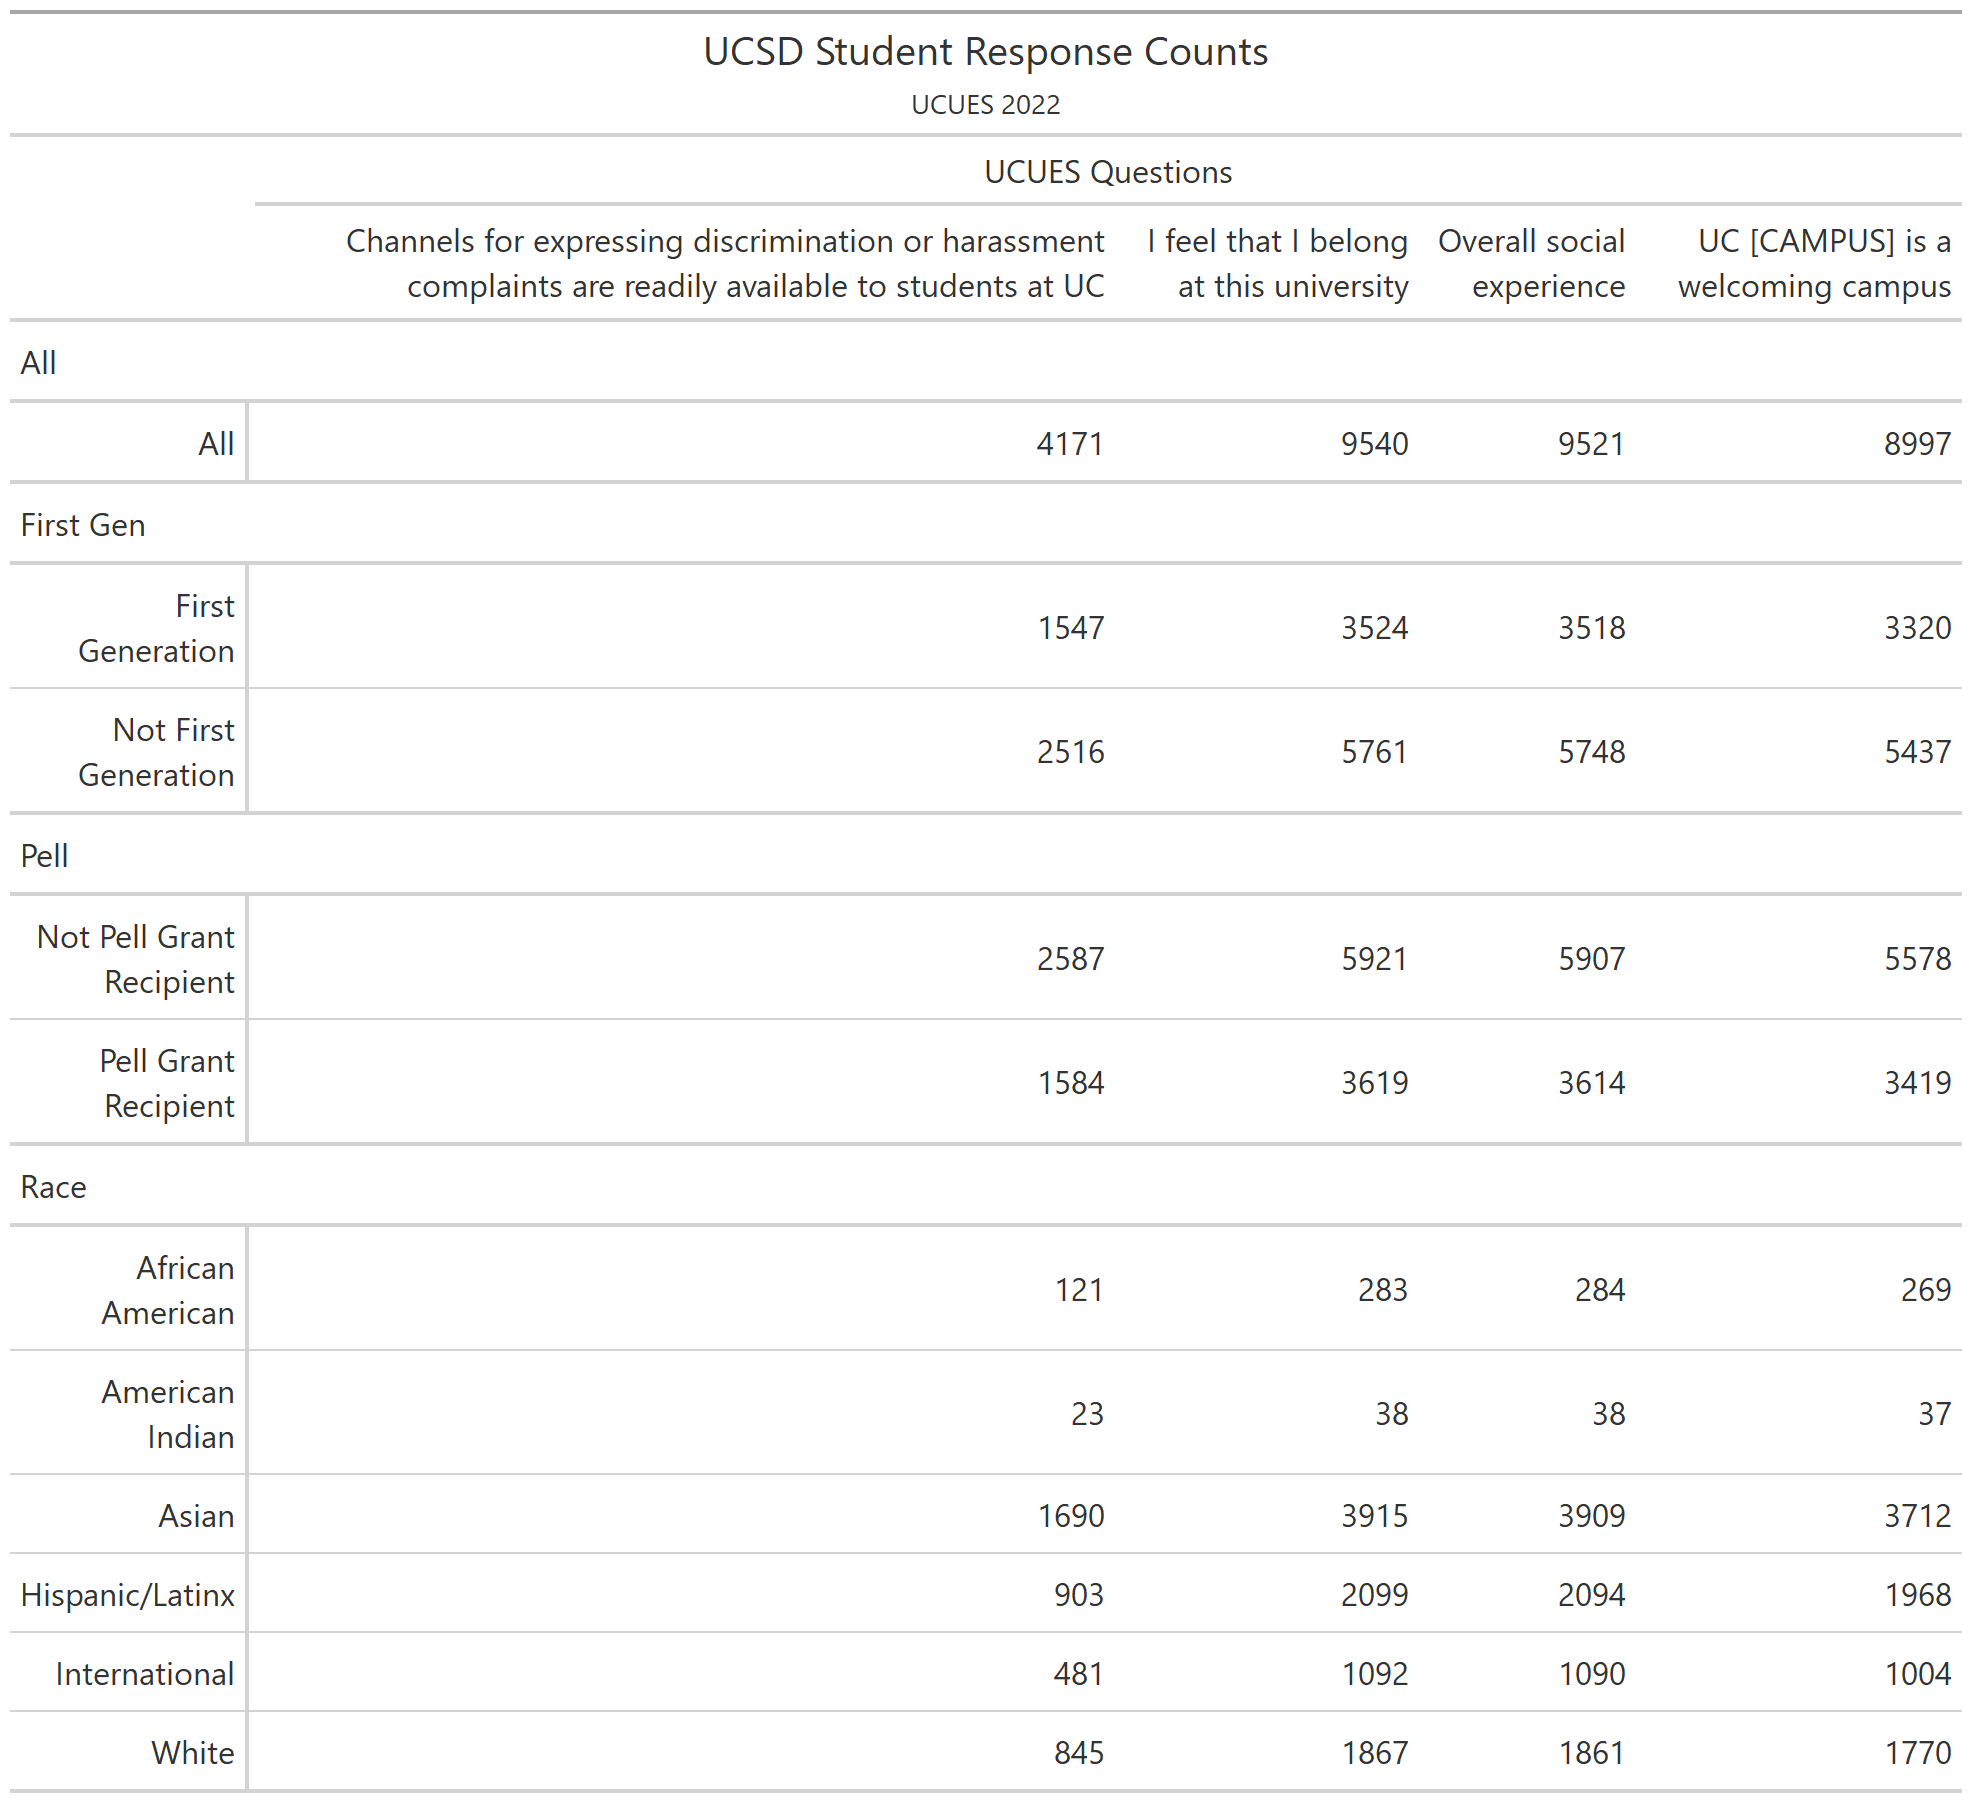
\includegraphics{./C4_Mentoring_Coaching_and_Advising_files/figure-pdf/rr_ug_gt-1.png}

\hypertarget{ucgses-1}{%
\subsection{UCGSES}\label{ucgses-1}}

\includegraphics{./C4_Mentoring_Coaching_and_Advising_files/figure-pdf/rr_grad_gt-1.png}

\bookmarksetup{startatroot}

\hypertarget{sense-of-belonging}{%
\chapter{Sense of Belonging}\label{sense-of-belonging}}

\hypertarget{i-feel-i-belong-at-this-university}{%
\subsection{I feel I belong at this
University}\label{i-feel-i-belong-at-this-university}}

\includegraphics{./C5_Sense_files/figure-pdf/belong_2022-1.pdf}

\hypertarget{i-feel-valued-as-an-individual}{%
\subsection{I feel valued as an
individual}\label{i-feel-valued-as-an-individual}}

\includegraphics{./C5_Sense_files/figure-pdf/valued_2022-1.pdf}

\hypertarget{rate-your-overall-social-experience}{%
\subsection{Rate your Overall Social
Experience}\label{rate-your-overall-social-experience}}

\includegraphics{./C5_Sense_files/figure-pdf/social_ex-1.pdf}

\hypertarget{uc-campus-is-welcoming}{%
\subsection{UC campus is Welcoming}\label{uc-campus-is-welcoming}}

\includegraphics{./C5_Sense_files/figure-pdf/welcome_2022-1.pdf}

\includegraphics{./C5_Sense_files/figure-pdf/climate_edi_2022-1.pdf}

\hypertarget{channels-for-addressing-discrimination}{%
\subsection{Channels for addressing
discrimination}\label{channels-for-addressing-discrimination}}

\includegraphics{./C5_Sense_files/figure-pdf/channel_dis-1.pdf}

\hypertarget{graduate-students-ucgses-1}{%
\section{Graduate Students (UCGSES)}\label{graduate-students-ucgses-1}}

\hypertarget{i-feel-included-by-my-peers}{%
\subsection{``I feel included by my
peers''}\label{i-feel-included-by-my-peers}}

\includegraphics{./C5_Sense_files/figure-pdf/include_peers-1.pdf}

\hypertarget{i-feel-included-by-the-administration-and-staff}{%
\subsection{I feel included by\ldots{} the administration and
staff''}\label{i-feel-included-by-the-administration-and-staff}}

\includegraphics{./C5_Sense_files/figure-pdf/include_admin-1.pdf}

\#\#\#I feel included by the faculty

\includegraphics{./C5_Sense_files/figure-pdf/include_fac-1.pdf}

\hypertarget{response-rates-2}{%
\section{Response Rates}\label{response-rates-2}}

\hypertarget{ucues-2}{%
\subsubsection{UCUES}\label{ucues-2}}

\includegraphics{./C5_Sense_files/figure-pdf/rr_ug_gt-1.png}

\hypertarget{ucgses-2}{%
\subsection{UCGSES}\label{ucgses-2}}

\includegraphics{./C5_Sense_files/figure-pdf/rr_grad_gt-1.png}

\bookmarksetup{startatroot}

\hypertarget{summary}{%
\chapter{Summary}\label{summary}}

This is a placeholder for future content

\bookmarksetup{startatroot}

\hypertarget{references}{%
\chapter*{References}\label{references}}
\addcontentsline{toc}{chapter}{References}

\markboth{References}{References}

This is a placeholder for future content ::: \{\#refs\} :::



\end{document}
